\documentclass[1p]{elsarticle_modified}
%\bibliographystyle{elsarticle-num}

%\usepackage[colorlinks]{hyperref}
%\usepackage{abbrmath_seonhwa} %\Abb, \Ascr, \Acal ,\Abf, \Afrak
\usepackage{amsfonts}
\usepackage{amssymb}
\usepackage{amsmath}
\usepackage{amsthm}
\usepackage{scalefnt}
\usepackage{amsbsy}
\usepackage{kotex}
\usepackage{caption}
\usepackage{subfig}
\usepackage{color}
\usepackage{graphicx}
\usepackage{xcolor} %% white, black, red, green, blue, cyan, magenta, yellow
\usepackage{float}
\usepackage{setspace}
\usepackage{hyperref}

\usepackage{tikz}
\usetikzlibrary{arrows}

\usepackage{multirow}
\usepackage{array} % fixed length table
\usepackage{hhline}

%%%%%%%%%%%%%%%%%%%%%
\makeatletter
\renewcommand*\env@matrix[1][\arraystretch]{%
	\edef\arraystretch{#1}%
	\hskip -\arraycolsep
	\let\@ifnextchar\new@ifnextchar
	\array{*\c@MaxMatrixCols c}}
\makeatother %https://tex.stackexchange.com/questions/14071/how-can-i-increase-the-line-spacing-in-a-matrix
%%%%%%%%%%%%%%%

\usepackage[normalem]{ulem}

\newcommand{\msout}[1]{\ifmmode\text{\sout{\ensuremath{#1}}}\else\sout{#1}\fi}
%SOURCE: \msout is \stkout macro in https://tex.stackexchange.com/questions/20609/strikeout-in-math-mode

\newcommand{\cancel}[1]{
	\ifmmode
	{\color{red}\msout{#1}}
	\else
	{\color{red}\sout{#1}}
	\fi
}

\newcommand{\add}[1]{
	{\color{blue}\uwave{#1}}
}

\newcommand{\replace}[2]{
	\ifmmode
	{\color{red}\msout{#1}}{\color{blue}\uwave{#2}}
	\else
	{\color{red}\sout{#1}}{\color{blue}\uwave{#2}}
	\fi
}

\newcommand{\Sol}{\mathcal{S}} %segment
\newcommand{\D}{D} %diagram
\newcommand{\A}{\mathcal{A}} %arc


%%%%%%%%%%%%%%%%%%%%%%%%%%%%%5 test

\def\sl{\operatorname{\textup{SL}}(2,\Cbb)}
\def\psl{\operatorname{\textup{PSL}}(2,\Cbb)}
\def\quan{\mkern 1mu \triangleright \mkern 1mu}

\theoremstyle{definition}
\newtheorem{thm}{Theorem}[section]
\newtheorem{prop}[thm]{Proposition}
\newtheorem{lem}[thm]{Lemma}
\newtheorem{ques}[thm]{Question}
\newtheorem{cor}[thm]{Corollary}
\newtheorem{defn}[thm]{Definition}
\newtheorem{exam}[thm]{Example}
\newtheorem{rmk}[thm]{Remark}
\newtheorem{alg}[thm]{Algorithm}

\newcommand{\I}{\sqrt{-1}}
\begin{document}

%\begin{frontmatter}
%
%\title{Boundary parabolic representations of knots up to 8 crossings}
%
%%% Group authors per affiliation:
%\author{Yunhi Cho} 
%\address{Department of Mathematics, University of Seoul, Seoul, Korea}
%\ead{yhcho@uos.ac.kr}
%
%
%\author{Seonhwa Kim} %\fnref{s_kim}}
%\address{Center for Geometry and Physics, Institute for Basic Science, Pohang, 37673, Korea}
%\ead{ryeona17@ibs.re.kr}
%
%\author{Hyuk Kim}
%\address{Department of Mathematical Sciences, Seoul National University, Seoul 08826, Korea}
%\ead{hyukkim@snu.ac.kr}
%
%\author{Seokbeom Yoon}
%\address{Department of Mathematical Sciences, Seoul National University, Seoul, 08826,  Korea}
%\ead{sbyoon15@snu.ac.kr}
%
%\begin{abstract}
%We find all boundary parabolic representation of knots up to 8 crossings.
%
%\end{abstract}
%\begin{keyword}
%    \MSC[2010] 57M25 
%\end{keyword}
%
%\end{frontmatter}

%\linenumbers
%\tableofcontents
%
\newcommand\colored[1]{\textcolor{white}{\rule[-0.35ex]{0.8em}{1.4ex}}\kern-0.8em\color{red} #1}%
%\newcommand\colored[1]{\textcolor{white}{ #1}\kern-2.17ex	\textcolor{white}{ #1}\kern-1.81ex	\textcolor{white}{ #1}\kern-2.15ex\color{red}#1	}

{\Large $\underline{12a_{0383}~(K12a_{0383})}$}

\setlength{\tabcolsep}{10pt}
\renewcommand{\arraystretch}{1.6}
\vspace{1cm}\begin{tabular}{m{100pt}>{\centering\arraybackslash}m{274pt}}
\multirow{5}{120pt}{
	\centering
	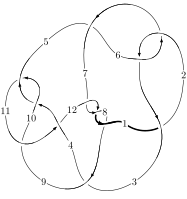
\includegraphics[width=112pt]{../../../GIT/diagram.site/Diagrams/png/1184_12a_0383.png}\\
\ \ \ A knot diagram\footnotemark}&
\allowdisplaybreaks
\textbf{Linearized knot diagam} \\
\cline{2-2}
 &
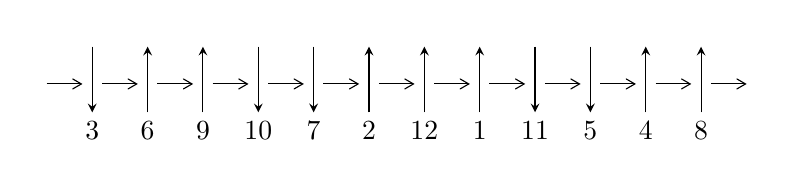
\begin{tikzpicture}[x=20pt, y=17pt]
	% nodes
	\node (C0) at (0, 0) {};
	\node (C1) at (1, 0) {};
	\node (C1U) at (1, +1) {};
	\node (C1D) at (1, -1) {3};

	\node (C2) at (2, 0) {};
	\node (C2U) at (2, +1) {};
	\node (C2D) at (2, -1) {6};

	\node (C3) at (3, 0) {};
	\node (C3U) at (3, +1) {};
	\node (C3D) at (3, -1) {9};

	\node (C4) at (4, 0) {};
	\node (C4U) at (4, +1) {};
	\node (C4D) at (4, -1) {10};

	\node (C5) at (5, 0) {};
	\node (C5U) at (5, +1) {};
	\node (C5D) at (5, -1) {7};

	\node (C6) at (6, 0) {};
	\node (C6U) at (6, +1) {};
	\node (C6D) at (6, -1) {2};

	\node (C7) at (7, 0) {};
	\node (C7U) at (7, +1) {};
	\node (C7D) at (7, -1) {12};

	\node (C8) at (8, 0) {};
	\node (C8U) at (8, +1) {};
	\node (C8D) at (8, -1) {1};

	\node (C9) at (9, 0) {};
	\node (C9U) at (9, +1) {};
	\node (C9D) at (9, -1) {11};

	\node (C10) at (10, 0) {};
	\node (C10U) at (10, +1) {};
	\node (C10D) at (10, -1) {5};

	\node (C11) at (11, 0) {};
	\node (C11U) at (11, +1) {};
	\node (C11D) at (11, -1) {4};

	\node (C12) at (12, 0) {};
	\node (C12U) at (12, +1) {};
	\node (C12D) at (12, -1) {8};
	\node (C13) at (13, 0) {};

	% arrows
	\draw[->,>={angle 60}]
	(C0) edge (C1) (C1) edge (C2) (C2) edge (C3) (C3) edge (C4) (C4) edge (C5) (C5) edge (C6) (C6) edge (C7) (C7) edge (C8) (C8) edge (C9) (C9) edge (C10) (C10) edge (C11) (C11) edge (C12) (C12) edge (C13) ;	\draw[->,>=stealth]
	(C1U) edge (C1D) (C2D) edge (C2U) (C3D) edge (C3U) (C4U) edge (C4D) (C5U) edge (C5D) (C6D) edge (C6U) (C7D) edge (C7U) (C8D) edge (C8U) (C9U) edge (C9D) (C10U) edge (C10D) (C11D) edge (C11U) (C12D) edge (C12U) ;
	\end{tikzpicture} \\
\hhline{~~} \\& 
\textbf{Solving Sequence} \\ \cline{2-2} 
 &
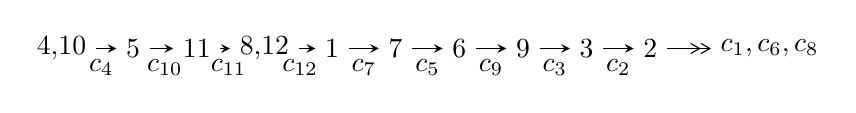
\begin{tikzpicture}[x=23pt, y=7pt]
	% node
	\node (A0) at (-1/8, 0) {4,10};
	\node (A1) at (1, 0) {5};
	\node (A2) at (2, 0) {11};
	\node (A3) at (49/16, 0) {8,12};
	\node (A4) at (33/8, 0) {1};
	\node (A5) at (41/8, 0) {7};
	\node (A6) at (49/8, 0) {6};
	\node (A7) at (57/8, 0) {9};
	\node (A8) at (65/8, 0) {3};
	\node (A9) at (73/8, 0) {2};
	\node (C1) at (1/2, -1) {$c_{4}$};
	\node (C2) at (3/2, -1) {$c_{10}$};
	\node (C3) at (5/2, -1) {$c_{11}$};
	\node (C4) at (29/8, -1) {$c_{12}$};
	\node (C5) at (37/8, -1) {$c_{7}$};
	\node (C6) at (45/8, -1) {$c_{5}$};
	\node (C7) at (53/8, -1) {$c_{9}$};
	\node (C8) at (61/8, -1) {$c_{3}$};
	\node (C9) at (69/8, -1) {$c_{2}$};
	\node (A10) at (11, 0) {$c_{1},c_{6},c_{8}$};

	% edge
	\draw[->,>=stealth]	
	(A0) edge (A1) (A1) edge (A2) (A2) edge (A3) (A3) edge (A4) (A4) edge (A5) (A5) edge (A6) (A6) edge (A7) (A7) edge (A8) (A8) edge (A9) ;
	\draw[->>,>={angle 60}]	
	(A9) edge (A10);
\end{tikzpicture} \\ 

\end{tabular} \\

\footnotetext{
The image of knot diagram is generated by the software ``\textbf{Draw programme}" developed by Andrew Bartholomew(\url{http://www.layer8.co.uk/maths/draw/index.htm\#Running-draw}), where we modified some parts for our purpose(\url{https://github.com/CATsTAILs/LinksPainter}).
}\phantom \\ \newline 
\centering \textbf{Ideals for irreducible components\footnotemark of $X_{\text{par}}$} 
 
\begin{align*}
I^u_{1}&=\langle 
5.33267\times10^{48} u^{94}-1.54204\times10^{49} u^{93}+\cdots+2.05960\times10^{49} b-5.95868\times10^{49},\\
\phantom{I^u_{1}}&\phantom{= \langle  }3.22494\times10^{49} u^{94}-8.97885\times10^{49} u^{93}+\cdots+2.05960\times10^{49} a-1.16528\times10^{50},\;u^{95}- u^{94}+\cdots+4 u-4\rangle \\
I^u_{2}&=\langle 
- u^2 a+u^3+2 b- u,\;-2 u^3 a-2 u^2 a+2 a^2-3 u^2+4 a-2 u+2,\;u^4-2 u^2+2\rangle \\
\\
I^v_{1}&=\langle 
a,\;b+v-1,\;v^2- v+1\rangle \\
\end{align*}
\raggedright * 3 irreducible components of $\dim_{\mathbb{C}}=0$, with total 105 representations.\\
\footnotetext{All coefficients of polynomials are rational numbers. But the coefficients are sometimes approximated in decimal forms when there is not enough margin.}
\newpage
\renewcommand{\arraystretch}{1}
\centering \section*{I. $I^u_{1}= \langle 5.33\times10^{48} u^{94}-1.54\times10^{49} u^{93}+\cdots+2.06\times10^{49} b-5.96\times10^{49},\;3.22\times10^{49} u^{94}-8.98\times10^{49} u^{93}+\cdots+2.06\times10^{49} a-1.17\times10^{50},\;u^{95}- u^{94}+\cdots+4 u-4 \rangle$}
\flushleft \textbf{(i) Arc colorings}\\
\begin{tabular}{m{7pt} m{180pt} m{7pt} m{180pt} }
\flushright $a_{4}=$&$\begin{pmatrix}1\\0\end{pmatrix}$ \\
\flushright $a_{10}=$&$\begin{pmatrix}0\\u\end{pmatrix}$ \\
\flushright $a_{5}=$&$\begin{pmatrix}1\\u^2\end{pmatrix}$ \\
\flushright $a_{11}=$&$\begin{pmatrix}- u\\- u^3+u\end{pmatrix}$ \\
\flushright $a_{8}=$&$\begin{pmatrix}-1.56581 u^{94}+4.35950 u^{93}+\cdots-9.90902 u+5.65780\\-0.258917 u^{94}+0.748705 u^{93}+\cdots-2.82171 u+2.89312\end{pmatrix}$ \\
\flushright $a_{12}=$&$\begin{pmatrix}- u^3\\- u^3+u\end{pmatrix}$ \\
\flushright $a_{1}=$&$\begin{pmatrix}1.56581 u^{94}-4.35950 u^{93}+\cdots+9.90902 u-5.65780\\1.44889 u^{94}-3.28930 u^{93}+\cdots+14.6163 u-8.28166\end{pmatrix}$ \\
\flushright $a_{7}=$&$\begin{pmatrix}-0.889379 u^{94}+2.45028 u^{93}+\cdots-3.06760 u+0.899810\\-0.103345 u^{94}+0.549833 u^{93}+\cdots+1.95019 u-0.333613\end{pmatrix}$ \\
\flushright $a_{6}=$&$\begin{pmatrix}2.23950 u^{94}-4.57433 u^{93}+\cdots+17.7650 u-8.24809\\-0.0601778 u^{94}+0.125437 u^{93}+\cdots+7.37150 u-3.67966\end{pmatrix}$ \\
\flushright $a_{9}=$&$\begin{pmatrix}u^3\\u^5- u^3+u\end{pmatrix}$ \\
\flushright $a_{3}=$&$\begin{pmatrix}u^8- u^6+u^4+1\\u^{10}-2 u^8+3 u^6-2 u^4+u^2\end{pmatrix}$ \\
\flushright $a_{2}=$&$\begin{pmatrix}0.848568 u^{94}-2.62471 u^{93}+\cdots-1.58235 u+0.136500\\1.77604 u^{94}-3.58781 u^{93}+\cdots+13.9026 u-7.98027\end{pmatrix}$\\&\end{tabular}
\flushleft \textbf{(ii) Obstruction class $= -1$}\\~\\
\flushleft \textbf{(iii) Cusp Shapes $= -0.840232 u^{94}+2.50685 u^{93}+\cdots-10.3269 u+17.5066$}\\~\\
\newpage\renewcommand{\arraystretch}{1}
\flushleft \textbf{(iv) u-Polynomials at the component}\newline \\
\begin{tabular}{m{50pt}|m{274pt}}
Crossings & \hspace{64pt}u-Polynomials at each crossing \\
\hline $$\begin{aligned}c_{1},c_{5}\end{aligned}$$&$\begin{aligned}
&u^{95}+30 u^{94}+\cdots-34 u-25
\end{aligned}$\\
\hline $$\begin{aligned}c_{2},c_{6}\end{aligned}$$&$\begin{aligned}
&u^{95}-2 u^{94}+\cdots+4 u+5
\end{aligned}$\\
\hline $$\begin{aligned}c_{3}\end{aligned}$$&$\begin{aligned}
&u^{95}+u^{94}+\cdots-82980 u-39988
\end{aligned}$\\
\hline $$\begin{aligned}c_{4},c_{10}\end{aligned}$$&$\begin{aligned}
&u^{95}- u^{94}+\cdots+4 u-4
\end{aligned}$\\
\hline $$\begin{aligned}c_{7},c_{8},c_{12}\end{aligned}$$&$\begin{aligned}
&u^{95}-3 u^{94}+\cdots-21 u-1
\end{aligned}$\\
\hline $$\begin{aligned}c_{9}\end{aligned}$$&$\begin{aligned}
&u^{95}+45 u^{94}+\cdots+80 u+16
\end{aligned}$\\
\hline $$\begin{aligned}c_{11}\end{aligned}$$&$\begin{aligned}
&u^{95}-3 u^{94}+\cdots+3028 u+44
\end{aligned}$\\
\hline
\end{tabular}\\~\\
\newpage\renewcommand{\arraystretch}{1}
\flushleft \textbf{(v) Riley Polynomials at the component}\newline \\
\begin{tabular}{m{50pt}|m{274pt}}
Crossings & \hspace{64pt}Riley Polynomials at each crossing \\
\hline $$\begin{aligned}c_{1},c_{5}\end{aligned}$$&$\begin{aligned}
&y^{95}+78 y^{94}+\cdots+72906 y-625
\end{aligned}$\\
\hline $$\begin{aligned}c_{2},c_{6}\end{aligned}$$&$\begin{aligned}
&y^{95}+30 y^{94}+\cdots-34 y-25
\end{aligned}$\\
\hline $$\begin{aligned}c_{3}\end{aligned}$$&$\begin{aligned}
&y^{95}-45 y^{94}+\cdots-7805590896 y-1599040144
\end{aligned}$\\
\hline $$\begin{aligned}c_{4},c_{10}\end{aligned}$$&$\begin{aligned}
&y^{95}-45 y^{94}+\cdots+80 y-16
\end{aligned}$\\
\hline $$\begin{aligned}c_{7},c_{8},c_{12}\end{aligned}$$&$\begin{aligned}
&y^{95}-95 y^{94}+\cdots+7 y-1
\end{aligned}$\\
\hline $$\begin{aligned}c_{9}\end{aligned}$$&$\begin{aligned}
&y^{95}+15 y^{94}+\cdots-1792 y-256
\end{aligned}$\\
\hline $$\begin{aligned}c_{11}\end{aligned}$$&$\begin{aligned}
&y^{95}+15 y^{94}+\cdots+8655568 y-1936
\end{aligned}$\\
\hline
\end{tabular}\\~\\
\newpage\flushleft \textbf{(vi) Complex Volumes and Cusp Shapes}
$$\begin{array}{c|c|c}  
\text{Solutions to }I^u_{1}& \I (\text{vol} + \sqrt{-1}CS) & \text{Cusp shape}\\
 \hline 
\begin{aligned}
u &= \phantom{-}1.00736\phantom{ +0.000000I} \\
a &= -3.08178\phantom{ +0.000000I} \\
b &= -1.34759\phantom{ +0.000000I}\end{aligned}
 & \phantom{-}2.55128\phantom{ +0.000000I} & \phantom{-0.000000 } 0 \\ \hline\begin{aligned}
u &= \phantom{-}0.906317 + 0.441368 I \\
a &= \phantom{-}0.010348 + 0.509452 I \\
b &= -0.555426 - 0.799270 I\end{aligned}
 & \phantom{-}1.64328 - 4.28747 I & \phantom{-0.000000 } 0 \\ \hline\begin{aligned}
u &= \phantom{-}0.906317 - 0.441368 I \\
a &= \phantom{-}0.010348 - 0.509452 I \\
b &= -0.555426 + 0.799270 I\end{aligned}
 & \phantom{-}1.64328 + 4.28747 I & \phantom{-0.000000 } 0 \\ \hline\begin{aligned}
u &= -0.924960 + 0.357461 I \\
a &= \phantom{-}3.42367 - 1.34161 I \\
b &= \phantom{-}0.64189 - 1.65711 I\end{aligned}
 & \phantom{-}0.71162 + 3.57000 I & \phantom{-0.000000 } 0 \\ \hline\begin{aligned}
u &= -0.924960 - 0.357461 I \\
a &= \phantom{-}3.42367 + 1.34161 I \\
b &= \phantom{-}0.64189 + 1.65711 I\end{aligned}
 & \phantom{-}0.71162 - 3.57000 I & \phantom{-0.000000 } 0 \\ \hline\begin{aligned}
u &= \phantom{-}0.634715 + 0.755350 I \\
a &= -0.338265 + 0.155743 I \\
b &= -2.09428 - 0.75954 I\end{aligned}
 & \phantom{-}12.0289 - 8.1472 I & \phantom{-0.000000 } 0 \\ \hline\begin{aligned}
u &= \phantom{-}0.634715 - 0.755350 I \\
a &= -0.338265 - 0.155743 I \\
b &= -2.09428 + 0.75954 I\end{aligned}
 & \phantom{-}12.0289 + 8.1472 I & \phantom{-0.000000 } 0 \\ \hline\begin{aligned}
u &= -1.010690 + 0.149709 I \\
a &= -0.690553 + 0.017344 I \\
b &= -0.652018 + 0.557209 I\end{aligned}
 & -0.044130 + 0.757058 I & \phantom{-0.000000 } 0 \\ \hline\begin{aligned}
u &= -1.010690 - 0.149709 I \\
a &= -0.690553 - 0.017344 I \\
b &= -0.652018 - 0.557209 I\end{aligned}
 & -0.044130 - 0.757058 I & \phantom{-0.000000 } 0 \\ \hline\begin{aligned}
u &= -0.606918 + 0.766435 I \\
a &= \phantom{-}0.336205 + 0.129569 I \\
b &= \phantom{-}2.16957 - 0.72542 I\end{aligned}
 & \phantom{-}12.72790 + 1.81622 I & \phantom{-0.000000 } 0\\
 \hline 
 \end{array}$$\newpage$$\begin{array}{c|c|c}  
\text{Solutions to }I^u_{1}& \I (\text{vol} + \sqrt{-1}CS) & \text{Cusp shape}\\
 \hline 
\begin{aligned}
u &= -0.606918 - 0.766435 I \\
a &= \phantom{-}0.336205 - 0.129569 I \\
b &= \phantom{-}2.16957 + 0.72542 I\end{aligned}
 & \phantom{-}12.72790 - 1.81622 I & \phantom{-0.000000 } 0 \\ \hline\begin{aligned}
u &= -0.887368 + 0.329507 I \\
a &= -0.140385 + 0.401837 I \\
b &= \phantom{-}0.065765 - 1.021190 I\end{aligned}
 & \phantom{-}0.884083 - 0.672783 I & \phantom{-0.000000 } 0 \\ \hline\begin{aligned}
u &= -0.887368 - 0.329507 I \\
a &= -0.140385 - 0.401837 I \\
b &= \phantom{-}0.065765 + 1.021190 I\end{aligned}
 & \phantom{-}0.884083 + 0.672783 I & \phantom{-0.000000 } 0 \\ \hline\begin{aligned}
u &= -1.006420 + 0.394031 I \\
a &= -0.708247 + 0.660629 I \\
b &= -0.288734 + 0.665580 I\end{aligned}
 & -1.66102 + 1.68609 I & \phantom{-0.000000 } 0 \\ \hline\begin{aligned}
u &= -1.006420 - 0.394031 I \\
a &= -0.708247 - 0.660629 I \\
b &= -0.288734 - 0.665580 I\end{aligned}
 & -1.66102 - 1.68609 I & \phantom{-0.000000 } 0 \\ \hline\begin{aligned}
u &= -0.397656 + 0.826000 I \\
a &= \phantom{-}0.298214 - 0.035388 I \\
b &= \phantom{-}2.52801 - 0.23592 I\end{aligned}
 & \phantom{-}11.54030 - 5.00777 I & \phantom{-}9.51836 + 0. I\phantom{ +0.000000I} \\ \hline\begin{aligned}
u &= -0.397656 - 0.826000 I \\
a &= \phantom{-}0.298214 + 0.035388 I \\
b &= \phantom{-}2.52801 + 0.23592 I\end{aligned}
 & \phantom{-}11.54030 + 5.00777 I & \phantom{-}9.51836 + 0. I\phantom{ +0.000000I} \\ \hline\begin{aligned}
u &= -1.066830 + 0.202202 I \\
a &= \phantom{-}3.41852 + 0.12892 I \\
b &= \phantom{-}1.71327 - 0.62864 I\end{aligned}
 & -1.00370 - 2.82785 I & \phantom{-0.000000 } 0 \\ \hline\begin{aligned}
u &= -1.066830 - 0.202202 I \\
a &= \phantom{-}3.41852 - 0.12892 I \\
b &= \phantom{-}1.71327 + 0.62864 I\end{aligned}
 & -1.00370 + 2.82785 I & \phantom{-0.000000 } 0 \\ \hline\begin{aligned}
u &= \phantom{-}0.374259 + 0.830094 I \\
a &= -0.291796 - 0.051261 I \\
b &= -2.53758 - 0.16345 I\end{aligned}
 & \phantom{-}10.5514 + 11.2514 I & \phantom{-}8.02405 - 5.87365 I\\
 \hline 
 \end{array}$$\newpage$$\begin{array}{c|c|c}  
\text{Solutions to }I^u_{1}& \I (\text{vol} + \sqrt{-1}CS) & \text{Cusp shape}\\
 \hline 
\begin{aligned}
u &= \phantom{-}0.374259 - 0.830094 I \\
a &= -0.291796 + 0.051261 I \\
b &= -2.53758 + 0.16345 I\end{aligned}
 & \phantom{-}10.5514 - 11.2514 I & \phantom{-}8.02405 + 5.87365 I \\ \hline\begin{aligned}
u &= \phantom{-}1.083220 + 0.170356 I \\
a &= \phantom{-}0.843048 - 0.029442 I \\
b &= \phantom{-}0.691071 + 0.592578 I\end{aligned}
 & -0.67601 + 4.68464 I & \phantom{-0.000000 } 0 \\ \hline\begin{aligned}
u &= \phantom{-}1.083220 - 0.170356 I \\
a &= \phantom{-}0.843048 + 0.029442 I \\
b &= \phantom{-}0.691071 - 0.592578 I\end{aligned}
 & -0.67601 - 4.68464 I & \phantom{-0.000000 } 0 \\ \hline\begin{aligned}
u &= -0.473838 + 0.746948 I \\
a &= \phantom{-}0.275238 + 0.041417 I \\
b &= \phantom{-}2.59227 - 0.60856 I\end{aligned}
 & \phantom{-}7.63537 - 1.35628 I & \phantom{-}10.70410 + 0.43713 I \\ \hline\begin{aligned}
u &= -0.473838 - 0.746948 I \\
a &= \phantom{-}0.275238 - 0.041417 I \\
b &= \phantom{-}2.59227 + 0.60856 I\end{aligned}
 & \phantom{-}7.63537 + 1.35628 I & \phantom{-}10.70410 - 0.43713 I \\ \hline\begin{aligned}
u &= -0.538924 + 0.699491 I \\
a &= \phantom{-}0.044940 + 0.780648 I \\
b &= -0.237329 + 0.267193 I\end{aligned}
 & \phantom{-}4.81550 + 4.38791 I & \phantom{-}7.51480 - 5.64431 I \\ \hline\begin{aligned}
u &= -0.538924 - 0.699491 I \\
a &= \phantom{-}0.044940 - 0.780648 I \\
b &= -0.237329 - 0.267193 I\end{aligned}
 & \phantom{-}4.81550 - 4.38791 I & \phantom{-}7.51480 + 5.64431 I \\ \hline\begin{aligned}
u &= \phantom{-}1.086530 + 0.303121 I \\
a &= \phantom{-}1.064310 + 0.311816 I \\
b &= \phantom{-}0.609869 + 0.789216 I\end{aligned}
 & -5.45074 - 0.28618 I & \phantom{-0.000000 } 0 \\ \hline\begin{aligned}
u &= \phantom{-}1.086530 - 0.303121 I \\
a &= \phantom{-}1.064310 - 0.311816 I \\
b &= \phantom{-}0.609869 - 0.789216 I\end{aligned}
 & -5.45074 + 0.28618 I & \phantom{-0.000000 } 0 \\ \hline\begin{aligned}
u &= \phantom{-}0.491332 + 0.709669 I \\
a &= -0.088786 + 0.815141 I \\
b &= \phantom{-}0.221359 + 0.254814 I\end{aligned}
 & \phantom{-}4.93908 + 1.43224 I & \phantom{-}8.06908 - 0.15779 I\\
 \hline 
 \end{array}$$\newpage$$\begin{array}{c|c|c}  
\text{Solutions to }I^u_{1}& \I (\text{vol} + \sqrt{-1}CS) & \text{Cusp shape}\\
 \hline 
\begin{aligned}
u &= \phantom{-}0.491332 - 0.709669 I \\
a &= -0.088786 - 0.815141 I \\
b &= \phantom{-}0.221359 - 0.254814 I\end{aligned}
 & \phantom{-}4.93908 - 1.43224 I & \phantom{-}8.06908 + 0.15779 I \\ \hline\begin{aligned}
u &= -0.403533 + 0.760268 I \\
a &= \phantom{-}0.267521 - 0.560532 I \\
b &= -1.022550 + 0.002110 I\end{aligned}
 & \phantom{-}4.09803 - 6.88748 I & \phantom{-}5.98803 + 5.67360 I \\ \hline\begin{aligned}
u &= -0.403533 - 0.760268 I \\
a &= \phantom{-}0.267521 + 0.560532 I \\
b &= -1.022550 - 0.002110 I\end{aligned}
 & \phantom{-}4.09803 + 6.88748 I & \phantom{-}5.98803 - 5.67360 I \\ \hline\begin{aligned}
u &= \phantom{-}0.435479 + 0.738565 I \\
a &= -0.340386 - 0.585466 I \\
b &= \phantom{-}0.976190 - 0.056007 I\end{aligned}
 & \phantom{-}4.63832 + 1.02745 I & \phantom{-}7.43624 - 0.48061 I \\ \hline\begin{aligned}
u &= \phantom{-}0.435479 - 0.738565 I \\
a &= -0.340386 + 0.585466 I \\
b &= \phantom{-}0.976190 + 0.056007 I\end{aligned}
 & \phantom{-}4.63832 - 1.02745 I & \phantom{-}7.43624 + 0.48061 I \\ \hline\begin{aligned}
u &= \phantom{-}0.512317 + 0.677131 I \\
a &= -0.239608 + 0.088733 I \\
b &= -2.59699 - 0.96252 I\end{aligned}
 & \phantom{-}4.13421 - 2.73861 I & \phantom{-}6.93438 + 3.68187 I \\ \hline\begin{aligned}
u &= \phantom{-}0.512317 - 0.677131 I \\
a &= -0.239608 - 0.088733 I \\
b &= -2.59699 + 0.96252 I\end{aligned}
 & \phantom{-}4.13421 + 2.73861 I & \phantom{-}6.93438 - 3.68187 I \\ \hline\begin{aligned}
u &= \phantom{-}0.400729 + 0.738352 I \\
a &= -0.245520 - 0.002118 I \\
b &= -2.82388 - 0.39352 I\end{aligned}
 & \phantom{-}3.54410 + 5.00424 I & \phantom{-}5.43059 - 4.10488 I \\ \hline\begin{aligned}
u &= \phantom{-}0.400729 - 0.738352 I \\
a &= -0.245520 + 0.002118 I \\
b &= -2.82388 + 0.39352 I\end{aligned}
 & \phantom{-}3.54410 - 5.00424 I & \phantom{-}5.43059 + 4.10488 I \\ \hline\begin{aligned}
u &= -1.102880 + 0.367477 I \\
a &= -0.344266 + 0.652241 I \\
b &= -0.121331 - 0.257026 I\end{aligned}
 & -2.50115 + 3.66582 I & \phantom{-0.000000 } 0\\
 \hline 
 \end{array}$$\newpage$$\begin{array}{c|c|c}  
\text{Solutions to }I^u_{1}& \I (\text{vol} + \sqrt{-1}CS) & \text{Cusp shape}\\
 \hline 
\begin{aligned}
u &= -1.102880 - 0.367477 I \\
a &= -0.344266 - 0.652241 I \\
b &= -0.121331 + 0.257026 I\end{aligned}
 & -2.50115 - 3.66582 I & \phantom{-0.000000 } 0 \\ \hline\begin{aligned}
u &= \phantom{-}1.098210 + 0.403695 I \\
a &= \phantom{-}1.22363 + 0.99160 I \\
b &= \phantom{-}0.259870 + 1.162480 I\end{aligned}
 & -2.86030 - 5.69493 I & \phantom{-0.000000 } 0 \\ \hline\begin{aligned}
u &= \phantom{-}1.098210 - 0.403695 I \\
a &= \phantom{-}1.22363 - 0.99160 I \\
b &= \phantom{-}0.259870 - 1.162480 I\end{aligned}
 & -2.86030 + 5.69493 I & \phantom{-0.000000 } 0 \\ \hline\begin{aligned}
u &= \phantom{-}1.054610 + 0.509286 I \\
a &= -0.029310 + 1.008540 I \\
b &= -0.757250 + 0.151276 I\end{aligned}
 & -0.74422 - 4.71578 I & \phantom{-0.000000 } 0 \\ \hline\begin{aligned}
u &= \phantom{-}1.054610 - 0.509286 I \\
a &= -0.029310 - 1.008540 I \\
b &= -0.757250 - 0.151276 I\end{aligned}
 & -0.74422 + 4.71578 I & \phantom{-0.000000 } 0 \\ \hline\begin{aligned}
u &= \phantom{-}0.968501 + 0.660448 I \\
a &= -0.27020 - 2.62071 I \\
b &= \phantom{-}1.67638 - 1.12462 I\end{aligned}
 & \phantom{-}11.03630 + 2.80075 I & \phantom{-0.000000 } 0 \\ \hline\begin{aligned}
u &= \phantom{-}0.968501 - 0.660448 I \\
a &= -0.27020 + 2.62071 I \\
b &= \phantom{-}1.67638 + 1.12462 I\end{aligned}
 & \phantom{-}11.03630 - 2.80075 I & \phantom{-0.000000 } 0 \\ \hline\begin{aligned}
u &= \phantom{-}0.713458 + 0.401814 I \\
a &= -2.02379 - 0.84772 I \\
b &= \phantom{-}0.143402 - 0.776861 I\end{aligned}
 & \phantom{-}2.20608 + 0.61401 I & \phantom{-}7.47589 + 1.44021 I \\ \hline\begin{aligned}
u &= \phantom{-}0.713458 - 0.401814 I \\
a &= -2.02379 + 0.84772 I \\
b &= \phantom{-}0.143402 + 0.776861 I\end{aligned}
 & \phantom{-}2.20608 - 0.61401 I & \phantom{-}7.47589 - 1.44021 I \\ \hline\begin{aligned}
u &= -1.025040 + 0.588917 I \\
a &= -0.364367 + 0.806386 I \\
b &= -0.196063 + 0.316449 I\end{aligned}
 & \phantom{-}3.37390 + 0.57283 I & \phantom{-0.000000 } 0\\
 \hline 
 \end{array}$$\newpage$$\begin{array}{c|c|c}  
\text{Solutions to }I^u_{1}& \I (\text{vol} + \sqrt{-1}CS) & \text{Cusp shape}\\
 \hline 
\begin{aligned}
u &= -1.025040 - 0.588917 I \\
a &= -0.364367 - 0.806386 I \\
b &= -0.196063 - 0.316449 I\end{aligned}
 & \phantom{-}3.37390 - 0.57283 I & \phantom{-0.000000 } 0 \\ \hline\begin{aligned}
u &= \phantom{-}1.175180 + 0.136636 I \\
a &= -3.02288 + 0.27797 I \\
b &= -1.86228 - 0.23548 I\end{aligned}
 & \phantom{-}6.23088 + 2.43913 I & \phantom{-0.000000 } 0 \\ \hline\begin{aligned}
u &= \phantom{-}1.175180 - 0.136636 I \\
a &= -3.02288 - 0.27797 I \\
b &= -1.86228 + 0.23548 I\end{aligned}
 & \phantom{-}6.23088 - 2.43913 I & \phantom{-0.000000 } 0 \\ \hline\begin{aligned}
u &= \phantom{-}1.040210 + 0.573890 I \\
a &= \phantom{-}0.06136 - 4.10879 I \\
b &= \phantom{-}2.46970 - 1.68079 I\end{aligned}
 & \phantom{-}2.56909 - 2.11335 I & \phantom{-0.000000 } 0 \\ \hline\begin{aligned}
u &= \phantom{-}1.040210 - 0.573890 I \\
a &= \phantom{-}0.06136 + 4.10879 I \\
b &= \phantom{-}2.46970 + 1.68079 I\end{aligned}
 & \phantom{-}2.56909 + 2.11335 I & \phantom{-0.000000 } 0 \\ \hline\begin{aligned}
u &= -1.094740 + 0.465086 I \\
a &= -0.46059 + 1.49298 I \\
b &= \phantom{-}0.548757 + 0.938106 I\end{aligned}
 & -2.46376 + 1.65618 I & \phantom{-0.000000 } 0 \\ \hline\begin{aligned}
u &= -1.094740 - 0.465086 I \\
a &= -0.46059 - 1.49298 I \\
b &= \phantom{-}0.548757 - 0.938106 I\end{aligned}
 & -2.46376 - 1.65618 I & \phantom{-0.000000 } 0 \\ \hline\begin{aligned}
u &= -0.993124 + 0.657208 I \\
a &= \phantom{-}0.10713 - 2.75718 I \\
b &= -1.80551 - 1.12242 I\end{aligned}
 & \phantom{-}11.57820 + 3.55082 I & \phantom{-0.000000 } 0 \\ \hline\begin{aligned}
u &= -0.993124 - 0.657208 I \\
a &= \phantom{-}0.10713 + 2.75718 I \\
b &= -1.80551 + 1.12242 I\end{aligned}
 & \phantom{-}11.57820 - 3.55082 I & \phantom{-0.000000 } 0 \\ \hline\begin{aligned}
u &= -1.184950 + 0.164320 I \\
a &= \phantom{-}3.03036 + 0.36882 I \\
b &= \phantom{-}1.92298 - 0.26030 I\end{aligned}
 & \phantom{-}5.34278 - 8.49470 I & \phantom{-0.000000 } 0\\
 \hline 
 \end{array}$$\newpage$$\begin{array}{c|c|c}  
\text{Solutions to }I^u_{1}& \I (\text{vol} + \sqrt{-1}CS) & \text{Cusp shape}\\
 \hline 
\begin{aligned}
u &= -1.184950 - 0.164320 I \\
a &= \phantom{-}3.03036 - 0.36882 I \\
b &= \phantom{-}1.92298 + 0.26030 I\end{aligned}
 & \phantom{-}5.34278 + 8.49470 I & \phantom{-0.000000 } 0 \\ \hline\begin{aligned}
u &= \phantom{-}0.022735 + 0.799824 I \\
a &= -0.015779 + 1.180600 I \\
b &= \phantom{-}0.009766 + 0.228412 I\end{aligned}
 & \phantom{-}5.58912 - 2.89667 I & \phantom{-}8.09026 + 2.86755 I \\ \hline\begin{aligned}
u &= \phantom{-}0.022735 - 0.799824 I \\
a &= -0.015779 - 1.180600 I \\
b &= \phantom{-}0.009766 - 0.228412 I\end{aligned}
 & \phantom{-}5.58912 + 2.89667 I & \phantom{-}8.09026 - 2.86755 I \\ \hline\begin{aligned}
u &= \phantom{-}1.054030 + 0.586974 I \\
a &= \phantom{-}0.368656 + 0.817874 I \\
b &= \phantom{-}0.189198 + 0.289956 I\end{aligned}
 & \phantom{-}3.27294 - 6.41274 I & \phantom{-0.000000 } 0 \\ \hline\begin{aligned}
u &= \phantom{-}1.054030 - 0.586974 I \\
a &= \phantom{-}0.368656 - 0.817874 I \\
b &= \phantom{-}0.189198 - 0.289956 I\end{aligned}
 & \phantom{-}3.27294 + 6.41274 I & \phantom{-0.000000 } 0 \\ \hline\begin{aligned}
u &= \phantom{-}1.117380 + 0.496941 I \\
a &= \phantom{-}0.365386 + 0.805784 I \\
b &= \phantom{-}0.098800 + 0.116809 I\end{aligned}
 & -1.61590 - 3.87546 I & \phantom{-0.000000 } 0 \\ \hline\begin{aligned}
u &= \phantom{-}1.117380 - 0.496941 I \\
a &= \phantom{-}0.365386 - 0.805784 I \\
b &= \phantom{-}0.098800 - 0.116809 I\end{aligned}
 & -1.61590 + 3.87546 I & \phantom{-0.000000 } 0 \\ \hline\begin{aligned}
u &= -1.103910 + 0.530704 I \\
a &= \phantom{-}0.304974 + 1.288360 I \\
b &= \phantom{-}1.144840 + 0.388579 I\end{aligned}
 & -3.92090 + 7.05751 I & \phantom{-0.000000 } 0 \\ \hline\begin{aligned}
u &= -1.103910 - 0.530704 I \\
a &= \phantom{-}0.304974 - 1.288360 I \\
b &= \phantom{-}1.144840 - 0.388579 I\end{aligned}
 & -3.92090 - 7.05751 I & \phantom{-0.000000 } 0 \\ \hline\begin{aligned}
u &= -1.069590 + 0.601922 I \\
a &= -0.70243 - 3.59618 I \\
b &= -2.53564 - 1.15017 I\end{aligned}
 & \phantom{-}5.86909 + 6.48356 I & \phantom{-0.000000 } 0\\
 \hline 
 \end{array}$$\newpage$$\begin{array}{c|c|c}  
\text{Solutions to }I^u_{1}& \I (\text{vol} + \sqrt{-1}CS) & \text{Cusp shape}\\
 \hline 
\begin{aligned}
u &= -1.069590 - 0.601922 I \\
a &= -0.70243 + 3.59618 I \\
b &= -2.53564 + 1.15017 I\end{aligned}
 & \phantom{-}5.86909 - 6.48356 I & \phantom{-0.000000 } 0 \\ \hline\begin{aligned}
u &= \phantom{-}1.084910 + 0.589192 I \\
a &= -0.469396 + 0.981001 I \\
b &= -1.280000 + 0.072585 I\end{aligned}
 & \phantom{-}2.72115 - 6.08579 I & \phantom{-0.000000 } 0 \\ \hline\begin{aligned}
u &= \phantom{-}1.084910 - 0.589192 I \\
a &= -0.469396 - 0.981001 I \\
b &= -1.280000 - 0.072585 I\end{aligned}
 & \phantom{-}2.72115 + 6.08579 I & \phantom{-0.000000 } 0 \\ \hline\begin{aligned}
u &= \phantom{-}1.098680 + 0.580905 I \\
a &= \phantom{-}1.39365 - 3.79866 I \\
b &= \phantom{-}2.94518 - 0.91850 I\end{aligned}
 & \phantom{-}1.49118 - 10.02840 I & \phantom{-0.000000 } 0 \\ \hline\begin{aligned}
u &= \phantom{-}1.098680 - 0.580905 I \\
a &= \phantom{-}1.39365 + 3.79866 I \\
b &= \phantom{-}2.94518 + 0.91850 I\end{aligned}
 & \phantom{-}1.49118 + 10.02840 I & \phantom{-0.000000 } 0 \\ \hline\begin{aligned}
u &= -1.103030 + 0.589063 I \\
a &= \phantom{-}0.529023 + 1.031450 I \\
b &= \phantom{-}1.333430 + 0.124726 I\end{aligned}
 & \phantom{-}2.03210 + 11.99530 I & \phantom{-0.000000 } 0 \\ \hline\begin{aligned}
u &= -1.103030 - 0.589063 I \\
a &= \phantom{-}0.529023 - 1.031450 I \\
b &= \phantom{-}1.333430 - 0.124726 I\end{aligned}
 & \phantom{-}2.03210 - 11.99530 I & \phantom{-0.000000 } 0 \\ \hline\begin{aligned}
u &= -0.612756 + 0.421387 I \\
a &= -0.078506 + 0.406547 I \\
b &= -0.368771 + 0.268543 I\end{aligned}
 & -0.54710 + 1.59075 I & \phantom{-}0.20356 - 5.77263 I \\ \hline\begin{aligned}
u &= -0.612756 - 0.421387 I \\
a &= -0.078506 - 0.406547 I \\
b &= -0.368771 - 0.268543 I\end{aligned}
 & -0.54710 - 1.59075 I & \phantom{-}0.20356 + 5.77263 I \\ \hline\begin{aligned}
u &= -1.197400 + 0.420007 I \\
a &= -0.424767 + 0.739784 I \\
b &= -0.256018 - 0.055789 I\end{aligned}
 & \phantom{-}1.92597 + 7.18036 I & \phantom{-0.000000 } 0\\
 \hline 
 \end{array}$$\newpage$$\begin{array}{c|c|c}  
\text{Solutions to }I^u_{1}& \I (\text{vol} + \sqrt{-1}CS) & \text{Cusp shape}\\
 \hline 
\begin{aligned}
u &= -1.197400 - 0.420007 I \\
a &= -0.424767 - 0.739784 I \\
b &= -0.256018 + 0.055789 I\end{aligned}
 & \phantom{-}1.92597 - 7.18036 I & \phantom{-0.000000 } 0 \\ \hline\begin{aligned}
u &= \phantom{-}1.194270 + 0.444123 I \\
a &= \phantom{-}0.417217 + 0.758396 I \\
b &= \phantom{-}0.241409 - 0.015942 I\end{aligned}
 & \phantom{-}2.09042 - 1.53105 I & \phantom{-0.000000 } 0 \\ \hline\begin{aligned}
u &= \phantom{-}1.194270 - 0.444123 I \\
a &= \phantom{-}0.417217 - 0.758396 I \\
b &= \phantom{-}0.241409 + 0.015942 I\end{aligned}
 & \phantom{-}2.09042 + 1.53105 I & \phantom{-0.000000 } 0 \\ \hline\begin{aligned}
u &= -0.295628 + 0.656995 I \\
a &= \phantom{-}0.233407 - 0.299723 I \\
b &= -0.836111 + 0.261445 I\end{aligned}
 & -1.62780 - 2.45074 I & -1.21302 + 4.58964 I \\ \hline\begin{aligned}
u &= -0.295628 - 0.656995 I \\
a &= \phantom{-}0.233407 + 0.299723 I \\
b &= -0.836111 - 0.261445 I\end{aligned}
 & -1.62780 + 2.45074 I & -1.21302 - 4.58964 I \\ \hline\begin{aligned}
u &= -1.125270 + 0.611077 I \\
a &= -1.42590 - 3.06717 I \\
b &= -2.60872 - 0.57625 I\end{aligned}
 & \phantom{-}9.36612 + 10.36270 I & \phantom{-0.000000 } 0 \\ \hline\begin{aligned}
u &= -1.125270 - 0.611077 I \\
a &= -1.42590 + 3.06717 I \\
b &= -2.60872 + 0.57625 I\end{aligned}
 & \phantom{-}9.36612 - 10.36270 I & \phantom{-0.000000 } 0 \\ \hline\begin{aligned}
u &= \phantom{-}1.135380 + 0.604145 I \\
a &= \phantom{-}1.59739 - 3.01825 I \\
b &= \phantom{-}2.65956 - 0.47148 I\end{aligned}
 & \phantom{-}8.2775 - 16.5876 I & \phantom{-0.000000 } 0 \\ \hline\begin{aligned}
u &= \phantom{-}1.135380 - 0.604145 I \\
a &= \phantom{-}1.59739 + 3.01825 I \\
b &= \phantom{-}2.65956 + 0.47148 I\end{aligned}
 & \phantom{-}8.2775 + 16.5876 I & \phantom{-0.000000 } 0 \\ \hline\begin{aligned}
u &= \phantom{-}0.403168 + 0.525934 I \\
a &= -0.565182 + 0.008925 I \\
b &= \phantom{-}0.488522 + 0.053919 I\end{aligned}
 & \phantom{-}1.114630 + 0.455666 I & \phantom{-}8.78049 - 1.93868 I\\
 \hline 
 \end{array}$$\newpage$$\begin{array}{c|c|c}  
\text{Solutions to }I^u_{1}& \I (\text{vol} + \sqrt{-1}CS) & \text{Cusp shape}\\
 \hline 
\begin{aligned}
u &= \phantom{-}0.403168 - 0.525934 I \\
a &= -0.565182 - 0.008925 I \\
b &= \phantom{-}0.488522 - 0.053919 I\end{aligned}
 & \phantom{-}1.114630 - 0.455666 I & \phantom{-}8.78049 + 1.93868 I \\ \hline\begin{aligned}
u &= \phantom{-}0.198800 + 0.620043 I \\
a &= -0.323351 + 1.208370 I \\
b &= \phantom{-}0.097754 + 0.148173 I\end{aligned}
 & \phantom{-}0.929200 - 0.474927 I & \phantom{-}3.13486 + 0.05006 I \\ \hline\begin{aligned}
u &= \phantom{-}0.198800 - 0.620043 I \\
a &= -0.323351 - 1.208370 I \\
b &= \phantom{-}0.097754 - 0.148173 I\end{aligned}
 & \phantom{-}0.929200 + 0.474927 I & \phantom{-}3.13486 - 0.05006 I \\ \hline\begin{aligned}
u &= -0.062646 + 0.547105 I \\
a &= \phantom{-}0.0309643 - 0.1334880 I \\
b &= -0.328550 + 0.882002 I\end{aligned}
 & \phantom{-}0.15393 + 2.22597 I & \phantom{-}0.01912 - 3.45127 I \\ \hline\begin{aligned}
u &= -0.062646 - 0.547105 I \\
a &= \phantom{-}0.0309643 + 0.1334880 I \\
b &= -0.328550 - 0.882002 I\end{aligned}
 & \phantom{-}0.15393 - 2.22597 I & \phantom{-}0.01912 + 3.45127 I\\
 \hline 
 \end{array}$$\newpage\newpage\renewcommand{\arraystretch}{1}
\centering \section*{II. $I^u_{2}= \langle - u^2 a+u^3+2 b- u,\;-2 u^3 a-2 u^2 a+2 a^2-3 u^2+4 a-2 u+2,\;u^4-2 u^2+2 \rangle$}
\flushleft \textbf{(i) Arc colorings}\\
\begin{tabular}{m{7pt} m{180pt} m{7pt} m{180pt} }
\flushright $a_{4}=$&$\begin{pmatrix}1\\0\end{pmatrix}$ \\
\flushright $a_{10}=$&$\begin{pmatrix}0\\u\end{pmatrix}$ \\
\flushright $a_{5}=$&$\begin{pmatrix}1\\u^2\end{pmatrix}$ \\
\flushright $a_{11}=$&$\begin{pmatrix}- u\\- u^3+u\end{pmatrix}$ \\
\flushright $a_{8}=$&$\begin{pmatrix}a\\\frac{1}{2} u^2 a-\frac{1}{2} u^3+\frac{1}{2} u\end{pmatrix}$ \\
\flushright $a_{12}=$&$\begin{pmatrix}- u^3\\- u^3+u\end{pmatrix}$ \\
\flushright $a_{1}=$&$\begin{pmatrix}- u^3+a\\\frac{1}{2} u^2 a-\frac{3}{2} u^3+\frac{3}{2} u\end{pmatrix}$ \\
\flushright $a_{7}=$&$\begin{pmatrix}- u^3+a\\\frac{1}{2} u^2 a-\frac{3}{2} u^3+\frac{3}{2} u\end{pmatrix}$ \\
\flushright $a_{6}=$&$\begin{pmatrix}\frac{1}{2} u^3 a-\frac{1}{2} u^3+\cdots+a+\frac{7}{2}\\\frac{1}{2} u^3 a-\frac{1}{2} u^3+\cdots+\frac{1}{2} u+1\end{pmatrix}$ \\
\flushright $a_{9}=$&$\begin{pmatrix}u^3\\u^3- u\end{pmatrix}$ \\
\flushright $a_{3}=$&$\begin{pmatrix}-1\\- u^2\end{pmatrix}$ \\
\flushright $a_{2}=$&$\begin{pmatrix}\frac{1}{2} u^2 a-\frac{3}{2} u^3+a+\frac{1}{2} u\\\frac{3}{2} u^2 a-2 u^3- a+\frac{5}{2} u\end{pmatrix}$\\&\end{tabular}
\flushleft \textbf{(ii) Obstruction class $= 1$}\\~\\
\flushleft \textbf{(iii) Cusp Shapes $= -2 u^2 a+2 u^3+4 u^2-2 u-4$}\\~\\
\newpage\renewcommand{\arraystretch}{1}
\flushleft \textbf{(iv) u-Polynomials at the component}\newline \\
\begin{tabular}{m{50pt}|m{274pt}}
Crossings & \hspace{64pt}u-Polynomials at each crossing \\
\hline $$\begin{aligned}c_{1},c_{2},c_{5}\end{aligned}$$&$\begin{aligned}
&(u^2- u+1)^4
\end{aligned}$\\
\hline $$\begin{aligned}c_{3},c_{11}\end{aligned}$$&$\begin{aligned}
&(u^4+2 u^2+2)^2
\end{aligned}$\\
\hline $$\begin{aligned}c_{4},c_{10}\end{aligned}$$&$\begin{aligned}
&(u^4-2 u^2+2)^2
\end{aligned}$\\
\hline $$\begin{aligned}c_{6}\end{aligned}$$&$\begin{aligned}
&(u^2+u+1)^4
\end{aligned}$\\
\hline $$\begin{aligned}c_{7},c_{8}\end{aligned}$$&$\begin{aligned}
&(u-1)^8
\end{aligned}$\\
\hline $$\begin{aligned}c_{9}\end{aligned}$$&$\begin{aligned}
&(u^2-2 u+2)^4
\end{aligned}$\\
\hline $$\begin{aligned}c_{12}\end{aligned}$$&$\begin{aligned}
&(u+1)^8
\end{aligned}$\\
\hline
\end{tabular}\\~\\
\newpage\renewcommand{\arraystretch}{1}
\flushleft \textbf{(v) Riley Polynomials at the component}\newline \\
\begin{tabular}{m{50pt}|m{274pt}}
Crossings & \hspace{64pt}Riley Polynomials at each crossing \\
\hline $$\begin{aligned}c_{1},c_{2},c_{5}\\c_{6}\end{aligned}$$&$\begin{aligned}
&(y^2+y+1)^4
\end{aligned}$\\
\hline $$\begin{aligned}c_{3},c_{11}\end{aligned}$$&$\begin{aligned}
&(y^2+2 y+2)^4
\end{aligned}$\\
\hline $$\begin{aligned}c_{4},c_{10}\end{aligned}$$&$\begin{aligned}
&(y^2-2 y+2)^4
\end{aligned}$\\
\hline $$\begin{aligned}c_{7},c_{8},c_{12}\end{aligned}$$&$\begin{aligned}
&(y-1)^8
\end{aligned}$\\
\hline $$\begin{aligned}c_{9}\end{aligned}$$&$\begin{aligned}
&(y^2+4)^4
\end{aligned}$\\
\hline
\end{tabular}\\~\\
\newpage\flushleft \textbf{(vi) Complex Volumes and Cusp Shapes}
$$\begin{array}{c|c|c}  
\text{Solutions to }I^u_{2}& \I (\text{vol} + \sqrt{-1}CS) & \text{Cusp shape}\\
 \hline 
\begin{aligned}
u &= \phantom{-}1.098680 + 0.455090 I \\
a &= -1.044230 + 0.410862 I \\
b &= -0.500000 - 0.866025 I\end{aligned}
 & -0.82247 - 5.69375 I & \phantom{-}2.00000 + 7.46410 I \\ \hline\begin{aligned}
u &= \phantom{-}1.098680 + 0.455090 I \\
a &= \phantom{-}0.68782 + 2.14291 I \\
b &= -0.500000 + 0.866025 I\end{aligned}
 & -0.82247 - 1.63398 I & \phantom{-}2.00000 + 0.53590 I \\ \hline\begin{aligned}
u &= \phantom{-}1.098680 - 0.455090 I \\
a &= -1.044230 - 0.410862 I \\
b &= -0.500000 + 0.866025 I\end{aligned}
 & -0.82247 + 5.69375 I & \phantom{-}2.00000 - 7.46410 I \\ \hline\begin{aligned}
u &= \phantom{-}1.098680 - 0.455090 I \\
a &= \phantom{-}0.68782 - 2.14291 I \\
b &= -0.500000 - 0.866025 I\end{aligned}
 & -0.82247 + 1.63398 I & \phantom{-}2.00000 - 0.53590 I \\ \hline\begin{aligned}
u &= -1.098680 + 0.455090 I \\
a &= \phantom{-}0.044228 - 0.589138 I \\
b &= -0.500000 - 0.866025 I\end{aligned}
 & -0.82247 + 1.63398 I & \phantom{-}2.00000 - 0.53590 I \\ \hline\begin{aligned}
u &= -1.098680 + 0.455090 I \\
a &= -1.68782 + 1.14291 I \\
b &= -0.500000 + 0.866025 I\end{aligned}
 & -0.82247 + 5.69375 I & \phantom{-}2.00000 - 7.46410 I \\ \hline\begin{aligned}
u &= -1.098680 - 0.455090 I \\
a &= \phantom{-}0.044228 + 0.589138 I \\
b &= -0.500000 + 0.866025 I\end{aligned}
 & -0.82247 - 1.63398 I & \phantom{-}2.00000 + 0.53590 I \\ \hline\begin{aligned}
u &= -1.098680 - 0.455090 I \\
a &= -1.68782 - 1.14291 I \\
b &= -0.500000 - 0.866025 I\end{aligned}
 & -0.82247 - 5.69375 I & \phantom{-}2.00000 + 7.46410 I\\
 \hline 
 \end{array}$$\newpage\newpage\renewcommand{\arraystretch}{1}
\centering \section*{III. $I^v_{1}= \langle a,\;b+v-1,\;v^2- v+1 \rangle$}
\flushleft \textbf{(i) Arc colorings}\\
\begin{tabular}{m{7pt} m{180pt} m{7pt} m{180pt} }
\flushright $a_{4}=$&$\begin{pmatrix}1\\0\end{pmatrix}$ \\
\flushright $a_{10}=$&$\begin{pmatrix}v\\0\end{pmatrix}$ \\
\flushright $a_{5}=$&$\begin{pmatrix}1\\0\end{pmatrix}$ \\
\flushright $a_{11}=$&$\begin{pmatrix}v\\0\end{pmatrix}$ \\
\flushright $a_{8}=$&$\begin{pmatrix}0\\- v+1\end{pmatrix}$ \\
\flushright $a_{12}=$&$\begin{pmatrix}v\\0\end{pmatrix}$ \\
\flushright $a_{1}=$&$\begin{pmatrix}v\\v-1\end{pmatrix}$ \\
\flushright $a_{7}=$&$\begin{pmatrix}- v\\- v+1\end{pmatrix}$ \\
\flushright $a_{6}=$&$\begin{pmatrix}0\\- v\end{pmatrix}$ \\
\flushright $a_{9}=$&$\begin{pmatrix}v\\0\end{pmatrix}$ \\
\flushright $a_{3}=$&$\begin{pmatrix}1\\0\end{pmatrix}$ \\
\flushright $a_{2}=$&$\begin{pmatrix}1\\v-1\end{pmatrix}$\\&\end{tabular}
\flushleft \textbf{(ii) Obstruction class $= 1$}\\~\\
\flushleft \textbf{(iii) Cusp Shapes $= -4 v+8$}\\~\\
\newpage\renewcommand{\arraystretch}{1}
\flushleft \textbf{(iv) u-Polynomials at the component}\newline \\
\begin{tabular}{m{50pt}|m{274pt}}
Crossings & \hspace{64pt}u-Polynomials at each crossing \\
\hline $$\begin{aligned}c_{1},c_{5},c_{6}\end{aligned}$$&$\begin{aligned}
&u^2- u+1
\end{aligned}$\\
\hline $$\begin{aligned}c_{2}\end{aligned}$$&$\begin{aligned}
&u^2+u+1
\end{aligned}$\\
\hline $$\begin{aligned}c_{3},c_{4},c_{9}\\c_{10},c_{11}\end{aligned}$$&$\begin{aligned}
&u^2
\end{aligned}$\\
\hline $$\begin{aligned}c_{7},c_{8}\end{aligned}$$&$\begin{aligned}
&(u+1)^2
\end{aligned}$\\
\hline $$\begin{aligned}c_{12}\end{aligned}$$&$\begin{aligned}
&(u-1)^2
\end{aligned}$\\
\hline
\end{tabular}\\~\\
\newpage\renewcommand{\arraystretch}{1}
\flushleft \textbf{(v) Riley Polynomials at the component}\newline \\
\begin{tabular}{m{50pt}|m{274pt}}
Crossings & \hspace{64pt}Riley Polynomials at each crossing \\
\hline $$\begin{aligned}c_{1},c_{2},c_{5}\\c_{6}\end{aligned}$$&$\begin{aligned}
&y^2+y+1
\end{aligned}$\\
\hline $$\begin{aligned}c_{3},c_{4},c_{9}\\c_{10},c_{11}\end{aligned}$$&$\begin{aligned}
&y^2
\end{aligned}$\\
\hline $$\begin{aligned}c_{7},c_{8},c_{12}\end{aligned}$$&$\begin{aligned}
&(y-1)^2
\end{aligned}$\\
\hline
\end{tabular}\\~\\
\newpage\flushleft \textbf{(vi) Complex Volumes and Cusp Shapes}
$$\begin{array}{c|c|c}  
\text{Solutions to }I^v_{1}& \I (\text{vol} + \sqrt{-1}CS) & \text{Cusp shape}\\
 \hline 
\begin{aligned}
v &= \phantom{-}0.500000 + 0.866025 I \\
a &= \phantom{-0.000000 } 0 \\
b &= \phantom{-}0.500000 - 0.866025 I\end{aligned}
 & \phantom{-}1.64493 + 2.02988 I & \phantom{-}6.00000 - 3.46410 I \\ \hline\begin{aligned}
v &= \phantom{-}0.500000 - 0.866025 I \\
a &= \phantom{-0.000000 } 0 \\
b &= \phantom{-}0.500000 + 0.866025 I\end{aligned}
 & \phantom{-}1.64493 - 2.02988 I & \phantom{-}6.00000 + 3.46410 I\\
 \hline 
 \end{array}$$\newpage
\newpage\renewcommand{\arraystretch}{1}
\centering \section*{ IV. u-Polynomials}
\begin{tabular}{m{50pt}|m{274pt}}
Crossings & \hspace{64pt}u-Polynomials at each crossing \\
\hline $$\begin{aligned}c_{1},c_{5}\end{aligned}$$&$\begin{aligned}
&((u^2- u+1)^5)(u^{95}+30 u^{94}+\cdots-34 u-25)
\end{aligned}$\\
\hline $$\begin{aligned}c_{2}\end{aligned}$$&$\begin{aligned}
&((u^2- u+1)^4)(u^2+u+1)(u^{95}-2 u^{94}+\cdots+4 u+5)
\end{aligned}$\\
\hline $$\begin{aligned}c_{3}\end{aligned}$$&$\begin{aligned}
&u^2(u^4+2 u^2+2)^2(u^{95}+u^{94}+\cdots-82980 u-39988)
\end{aligned}$\\
\hline $$\begin{aligned}c_{4},c_{10}\end{aligned}$$&$\begin{aligned}
&u^2(u^4-2 u^2+2)^2(u^{95}- u^{94}+\cdots+4 u-4)
\end{aligned}$\\
\hline $$\begin{aligned}c_{6}\end{aligned}$$&$\begin{aligned}
&(u^2- u+1)(u^2+u+1)^4(u^{95}-2 u^{94}+\cdots+4 u+5)
\end{aligned}$\\
\hline $$\begin{aligned}c_{7},c_{8}\end{aligned}$$&$\begin{aligned}
&((u-1)^8)(u+1)^2(u^{95}-3 u^{94}+\cdots-21 u-1)
\end{aligned}$\\
\hline $$\begin{aligned}c_{9}\end{aligned}$$&$\begin{aligned}
&u^2(u^2-2 u+2)^4(u^{95}+45 u^{94}+\cdots+80 u+16)
\end{aligned}$\\
\hline $$\begin{aligned}c_{11}\end{aligned}$$&$\begin{aligned}
&u^2(u^4+2 u^2+2)^2(u^{95}-3 u^{94}+\cdots+3028 u+44)
\end{aligned}$\\
\hline $$\begin{aligned}c_{12}\end{aligned}$$&$\begin{aligned}
&((u-1)^2)(u+1)^8(u^{95}-3 u^{94}+\cdots-21 u-1)
\end{aligned}$\\
\hline
\end{tabular}\newpage\renewcommand{\arraystretch}{1}
\centering \section*{ V. Riley Polynomials}
\begin{tabular}{m{50pt}|m{274pt}}
Crossings & \hspace{64pt}Riley Polynomials at each crossing \\
\hline $$\begin{aligned}c_{1},c_{5}\end{aligned}$$&$\begin{aligned}
&((y^2+y+1)^5)(y^{95}+78 y^{94}+\cdots+72906 y-625)
\end{aligned}$\\
\hline $$\begin{aligned}c_{2},c_{6}\end{aligned}$$&$\begin{aligned}
&((y^2+y+1)^5)(y^{95}+30 y^{94}+\cdots-34 y-25)
\end{aligned}$\\
\hline $$\begin{aligned}c_{3}\end{aligned}$$&$\begin{aligned}
&y^2(y^2+2 y+2)^4(y^{95}-45 y^{94}+\cdots-7.80559\times10^{9} y-1.59904\times10^{9})
\end{aligned}$\\
\hline $$\begin{aligned}c_{4},c_{10}\end{aligned}$$&$\begin{aligned}
&y^2(y^2-2 y+2)^4(y^{95}-45 y^{94}+\cdots+80 y-16)
\end{aligned}$\\
\hline $$\begin{aligned}c_{7},c_{8},c_{12}\end{aligned}$$&$\begin{aligned}
&((y-1)^{10})(y^{95}-95 y^{94}+\cdots+7 y-1)
\end{aligned}$\\
\hline $$\begin{aligned}c_{9}\end{aligned}$$&$\begin{aligned}
&y^2(y^2+4)^4(y^{95}+15 y^{94}+\cdots-1792 y-256)
\end{aligned}$\\
\hline $$\begin{aligned}c_{11}\end{aligned}$$&$\begin{aligned}
&y^2(y^2+2 y+2)^4(y^{95}+15 y^{94}+\cdots+8655568 y-1936)
\end{aligned}$\\
\hline
\end{tabular}
\vskip 2pc
\end{document}